\chapter{Product}\label{chap:product}

\section{Implementation of the prototype}

\cite{brandt2008opportunistic}

\section{Programming language choice}

% TODO: Table of languages

\subsection{Functional programming paradigms}

% FUNCTIONAL PROGRAMMING

\cite{hughes1989functional}

% CLOJURE

\cite{halloway2009programming, fogus2011joy}

% Clojure parallelization

\cite{kraus2009multi}

% PHP vs Clojure

\subsection{Web programming with functional languages}

% Similarities to JavaScript (and it's popularity)

\section{Prototype rewrite in LISP}


\subsection{Routing}

% TODO: No more 1-1 mapping of file -> URL.

\lstset{language=Clojure}
\begin{lstlisting}[label=lst:router,caption={
      [Application ring handler routes]
      Application ring handler routes, taken from \texttt{middleware.clj}.}]
(defroutes routes
  (GET  ["/"]                      [:as request] (index/GET       request))
  (GET  ["/advanced"]              [:as request] (advanced/GET    request))
  (GET  ["/r/:id.json", :id id-re] [:as request] (api/r           request))
  (GET  ["/r/:id",      :id id-re] [:as request] (record/GET      request))
  (GET  ["/d"]                     [:as request] (download/GET    request))
  (GET  ["/s"]                     [:as request] (search/GET      request))
  (POST ["/s"]                     [:as request] (search/POST     request))
  (GET  ["/s.json"]                [:as request] (api/s           request))
  (GET  ["/blast"]                 [:as request] (blast/GET       request))
  (GET  ["/login"]                 [:as request] (login/GET       request))
  (POST ["/login"]                 [:as request] (login/POST      request))
  (GET  ["/logout"]                [:as request] (logout/GET      request))
  (GET  ["/upload"]                [:as request] (upload/GET      request))
  (POST ["/upload"]                [:as request] (upload/POST     request))
  (GET  ["/api/s"]                 [:as request] (api/s           request))
  (GET  ["/api/r/:id",  :id id-re] [:as request] (api/r           request))
  (GET  ["/api/ac"]                [:as request] (api/ac          request))
  (GET  ["/api/ping"]              [:as request] (api/ping        request))
  (route/resources "/")
  (route/not-found (ui/page-404)))
\end{lstlisting}


\section{Persistent storage}

% TODO: Replicate errors in dataset

\subsection{Yet Another Protein Schema}


%%%%%%%%%%%%%%%%%%%%%%%%
%% Table: yaps-schema %%
%%%%%%%%%%%%%%%%%%%%%%%%
\newpage
\begin{table}[H]
\centering
\begin{tabular}{| l | l | l |}
\hline
\textbf{Field} & \textbf{Type} & \textbf{Description}\\
\hline
\textbf{id} & \textit{varchar(11)*} & Unique record identifier\\
\textbf{Protein-Names} & \textit{varchar} & Forward slash (``/'') delimited names\\
\textbf{EC} & \textit{varchar} & Enzyme commission number\\
\textbf{Source} & \textit{varchar} & Protein source\\
\textbf{Location} & \textit{varchar} & Organ and/or Subcellular location\\
\textbf{MW-Min} & \textit{varchar} & Molecular weight minimum\\
\textbf{MW-Max} & \textit{varchar} & Molecular weight maximum\\
\textbf{Subunit-No} & \textit{varchar} & Subunit number\\
\textbf{Subunit-MW} & \textit{varchar} & Subunit molecular weight\\
\textbf{No-Of-Iso-Enzymes} & \textit{varchar} & Number of iso-enzymes\\
\textbf{pI-Min} & \textit{varchar} & Isoelectric point minimum\\
\textbf{pI-Max} & \textit{varchar} & Isoelectric point maximum\\
\textbf{pI-Major-Component} & \textit{varchar} & Isoelectric point of major component\\
\textbf{Temperature-Min} & \textit{varchar} & Experimental temperature minimum\\
\textbf{Temperature-Max} & \textit{varchar} & Experimental temperature maximum\\
\textbf{Method} & \textit{varchar} & Experimental method\\
\textbf{Full-Text} & \textit{varchar} & URL of full text citation\\
\textbf{Abstract-Only} & \textit{varchar} & URL of abstract-only citation\\
\textbf{PubMed} & \textit{varchar} & URL of PubMed article\\
\textbf{Species-Taxonomy} & \textit{varchar} & URL of species taxonomy reference\\
\textbf{Protein-Sequence} & \textit{varchar} & URL of protein sequence reference\\
\textbf{Notes} & \textit{varchar} & Notes and annotations\\
\textbf{Sequence-Name} & \textit{varchar} & FASTA sequence description\\
\textbf{Sequence-Data} & \textit{varchar} & FASTA sequence data\\
\textbf{real\_ec1} & \textit{integer} & Numerical first component of EC\\
\textbf{real\_ec2} & \textit{integer} & Numerical second component of EC\\
\textbf{real\_ec3} & \textit{integer} & Numerical third component of EC\\
\textbf{real\_ec4} & \textit{integer} & Numerical four component of EC\\
\textbf{real\_mw\_min} & \textit{real} & Numerical molecular weight minimum\\
\textbf{real\_mw\_max} & \textit{real} & Numerical molecular weight maximum\\
\textbf{real\_pi\_min} & \textit{real} & Numerical isoelectric point minimum\\
\textbf{real\_pi\_max} & \textit{real} & Numerical isoelectric point maximum\\
\textbf{real\_temp\_min} & \textit{real} & Numerical temperature minimum\\
\textbf{real\_temp\_max} & \textit{real} & Numerical temperature maximum\\
\textbf{Created-At} & \textit{timestamp*} & Timestamp of dataset creation\\
\hline
\end{tabular}
\caption[YAPS schema]
        {YAPS schema definition. Fields with an asterisk (*) are
         mandatory, other fields may be null.}
\label{tab:yaps-schema}
\end{table}


% TODO: derived fields (id, Created-At, all integer+real)


%%%%%%%%%%%%%%%%%%%%%%%%%%%
%% Listing: yaps-example %%
%%%%%%%%%%%%%%%%%%%%%%%%%%%
\lstset{language=JavaScript}
\begin{lstlisting}[label=lst:yaps-example,caption={
      [Example YAPS encoded dataset]
      An example YAPS encoded dataset, containing a single record.}]
{
  "Encoding": "yaps",
  "Version": 4,
  "Date": "2014-04-20 02:29:48",
  "Author": "chris@vm-ubuntu",
  "Agent": "/home/chris/src/pip-db/tools/csv2yaps/csv2yaps.js",
  "Source": "/home/chris/dataset-test.txt",
  "No-Of-Records": 1,
  "Records": [
    {
      "Protein-Names": [
        "Acetoacetyl-CoA thiolase",
        "Acetyl-CoA acetyltransferase"
      ],
      "EC": "2.3.1.9",
      "Source": "Saccharomyces cerevisiae (Yeast)",
      "Location": "Cytosol",
      "MW-Min": "140000",
      "MW-Max": "140000",
      "No-Of-Iso-Enzymes": "1",
      "pI-Min": "5.3",
      "pI-Max": "5.3",
      "Temperature-Min": "4",
      "Temperature-Max": "4",
      "Method": "Isoelectric focusing",
      "Full-Text": "http://www.jbc.org/content/246/14/4424 ...",
      "PubMed": "http://www.ncbi.nlm.nih.gov/pubmed/557183 ...",
      "Species-Taxonomy": "http://www.ncbi.nlm.nih.gov/Tax ...",
      "Protein-Sequence": "http://www.uniprot.org/uniprot/ ...",
      "Sequence-Name": ">sp|P41338|THIL_YEAST Acetyl-CoA a ..."
      "Sequence-Data": "MSQNVYIVSTARTPIGSFQGSLSSKTAVELGAVA ..."
    }
}
\end{lstlisting}

\subsubsection*{Unique hash identification}

% TODO: Add collision probability calculation and entropy

\begin{verbatim}
(defn minihash [s]
  (subs (str->b64 (sha1 s)) 0 11))
\end{verbatim}


\subsubsection*{Protein sequence crawling}

% TODO: fetch-fasta


\subsubsection*{Version control}

% TODO: CSV


\section{Search engine design}

%%%%%%%%%%%%%%%%%%%%%%%%%%%%%
%% Table: query-components %%
%%%%%%%%%%%%%%%%%%%%%%%%%%%%%
\begin{table}[H]
\centering
\begin{tabular}{| c | c | l |}
\hline
\textbf{Family} & \textbf{Symbol} & \textbf{Definition}\\
\hline
& $id$ & Unique identifier\\
$N$ & $q_0 \ldots q_n$ & Any keywords\\
$N$ & $a_0 \ldots a_n$ & All keywords\\
$N$ & $n_0 \ldots n_n$ & Not keywords\\
$N$ & $eq$ & Exact phrase\\
$P$ & $p_l$, $p_h$ & Minimum and maximum isoelectric point\\
$P$ & $m_l$, $m_h$ & Minimum and maximum molecular weight\\
$P$ & $e_0$, $e_1$, $e_2$, $e_3$ & Enzyme commission number\\
$P$ & $l_s$ & Source location\\
$P$ & $l_l$ & Organ or sub-cellular location\\
$P$ & $f_n$ & FASTA sequence name\\
$P$ & $f_s$ & FASTA sequence string\\
$E$ & $m$ & Experimental method\\
$E$ & $t_l$, $t_h$ & Minimum and maximum experimental temperature\\
\hline
\end{tabular}
\caption[Query component symbols and their definitions]{Query component symbols and their definitions.}
\label{tab:query-components}
\end{table}


% TODO: example searches (and URLs) from appendix

\newpage

%%%%%%%%%%%%%%%%%%%%%%%%
%% Figure: query-tree %%
%%%%%%%%%%%%%%%%%%%%%%%%
\begin{figure}[t]
\centering
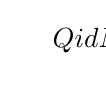
\begin{tikzpicture}
\tikzset{level distance=50pt, sibling distance=1.5pt}
  \Tree [.{$Q$}
    [.{$id$} ]
    [.{$N$}
      [.{$Q$}
        [. \node(q0){$q_0$}; ]
        [. \node(qn){$q_n$}; ]
      ]
      [.{$A$}
        [. \node(a0){$a_0$}; ]
        [. \node(an){$a_n$}; ]
      ]
      [. {$N$}
        [. \node(n0){$n_0$}; ]
        [. \node(nn){$n_n$}; ]
      ]
      [.{$eq$} ]
    ]
    [.{$P$}
      [.{$P$}
        [.{$p_l$} ]
        [.{$p_h$} ]
      ]
      [.{$M$}
        [.{$m_l$} ]
        [.{$m_h$} ]
      ]
      [.{$E$}
        [.{$e_0$} ]
        [.{$e_1$} ]
        [.{$e_2$} ]
        [.{$e_3$} ]
      ]
      [.{$L$}
        [.{$l_s$} ]
        [.{$l_l$} ]
      ]
      [.{$F$}
        [.{$f_n$} ]
        [.{$f_s$} ]
      ]
    ]
    [.{$E$}
      [.{$m$} ]
      [.{$T$}
        [. \node(tl){$t_l$}; ]
        [. \node(th){$t_h$}; ]
      ]
    ]
  ]
\begin{scope}[dashed]
\draw (a0)--(an);
\draw (n0)--(nn);
\draw (q0)--(qn);
\end{scope}
\end{tikzpicture}
\caption[Structure of the query tree for composing searches]
        {Structure of the query tree used for composing searches of
          the PIP-DB dataset. Leaf nodes represent properties. Nodes
          with an uppercase name denote compound AND conditionals.}
\label{fig:query-tree}
\end{figure}


%%%%%%%%%%%%%%%%%%%%%%%%%
%% Listing: query-tree %%
%%%%%%%%%%%%%%%%%%%%%%%%%
\lstset{language=Clojure}
\begin{lstlisting}[label=lst:query-tree,caption={
      [Clojure implementation of the query tree]
      Implementation of the query tree in Clojure, from the file
      \texttt{query.clj}. Note the flat query hierarchy and the
      use of the \texttt{for} macro for expanding multivalued
      queries.}]
(AND
 (EQ   {:field "id"            :value id :exact true})
 (for [word q]
   (EQ {:field "Protein-Names" :value word}))
 (for [word q_any]
   (EQ {:field "Protein-Names" :value word}))
 (for [word q_ne]
   (NE {:field "Protein-Names" :value word}))
 (EQ   {:field "Protein-Names" :value q_eq})
 (EQ   {:field "Source"        :value q_s})
 (EQ   {:field "Location"      :value q_l})
 (EQ   {:field "Method"        :value m})
 (EQ   {:field "Sequence-Name" :value seq})
 (GTE  {:field "real_pi_min"   :value pi_l})
 (LTE  {:field "real_pi_max"   :value pi_h})
 (GTE  {:field "real_mw_min"   :value mw_l})
 (LTE  {:field "real_mw_max"   :value mw_h})
 (GTE  {:field "real_temp_min" :value t_l})
 (LTE  {:field "real_temp_max" :value t_h})
 (EQ   {:field "real_ec1"      :value ec1 :numeric true})
 (EQ   {:field "real_ec2"      :value ec2 :numeric true})
 (EQ   {:field "real_ec3"      :value ec3 :numeric true})
 (EQ   {:field "real_ec4"      :value ec4 :numeric true}))
\end{lstlisting}


\subsection{Incorporating BLAST+ searching}

\newpage
\subsubsection*{Dynamic dispatcher}

%%%%%%%%%%%%%%%%%%%%%%%%%%%%%%%%
%% Listing: search-dispatcher %%
%%%%%%%%%%%%%%%%%%%%%%%%%%%%%%%%
\lstset{language=Clojure}
\begin{lstlisting}[label=lst:search-dispatcher,caption={
      [Search handler and dynamic dispatcher]
      Search handler and dynamic dispatcher. Accepting a request map,
      the search handler dispatches the appropriate search function
      (line \ref{lst:search-dispatcher-dispatch}), wrapping the
      results into a response map.}]
(defn search [request]
  (let [sequence     ((request :params) "seq")
        blast?       (not (str/blank? sequence))
        params       (request :params)
        headers      (request :headers)
        query-terms? (not (= (headers "x-pip-db-query-terms") "None"))
        records?     (not (= (headers "x-pip-db-records")     "None"))
(*@\label{lst:search-dispatcher-dispatch}@*)        matching-records    (if blast? (blast/search request)
                                       (db/search    request))
        no-records-searched (if blast? (blast/no-of-records)
                                       (db/no-of-records))]
    (merge
     (if records?
       (let [returned-records (take max-no-of-returned-records
                                    matching-records)]
         {:No-Of-Records-Returned  (count returned-records)
          :Records                  returned-records}))
     {:No-Of-Records-Matched       (count matching-records)
      :Max-No-of-Returned-Records   max-no-of-returned-records
      :No-Of-Records-Searched       no-records-searched}
     (if query-terms?
       {:Query-Terms               (dissoc params "seq_name")}))))
\end{lstlisting}

 The \texttt{params->str} function (line \ref{lst:db-search-str})
 converts a search parameter map into a structured query tree
 (figure~\ref{fig:query-tree}) and serialises it into an SQL select
 statement. This is used to generate a vector of record rows which are
 mapped over the \texttt{row->record} function (line
 \ref{lst:db-search-row}), converting them back into structured YAPS
 records.


%%%%%%%%%%%%%%%%%%%%%%%%
%% Listing: db-search %%
%%%%%%%%%%%%%%%%%%%%%%%%
\lstset{language=Clojure}
\begin{lstlisting}[label=lst:db-search,caption={
      [The \texttt{db} namespace search function]
      The \texttt{db} namespace search function.}]
(defn search [request]
(*@\label{lst:db-search-str}@*)  (let [query-str (params->str (request :params))]
(*@\label{lst:db-search-row}@*)    (map row->record (search-results query-str))))
\end{lstlisting}


The blast search function (Listing~\ref{lst:blast-search}) first
executes the \texttt{blastp} program with an appropriate environment
and input filtered from the request map (line
\ref{lst:blast-search-blastp}), and then maps the output of the
program into the function \texttt{result->records} which performs a
reverse lookup of the matched sequences and performs repeated database
searches for the matched records using the parameter map.


%%%%%%%%%%%%%%%%%%%%%%%%%%%
%% Listing: blast-search %%
%%%%%%%%%%%%%%%%%%%%%%%%%%%
\lstset{language=Clojure}
\begin{lstlisting}[label=lst:blast-search,caption={
      [The \texttt{blast} namespace search function]
      The \texttt{blast} namespace search function.}]
(defn search [request]
(*@\label{lst:blast-search-blastp}@*)  (let [results (blast-results ((request :params) "seq"))]
(*@\label{lst:blast-search-map}@*)    (flatten (map #(result->records request %) results))))
\end{lstlisting}

\newpage
Listing \ref{lst:blast-search-wrapper} shows the implementation of the
\texttt{results->records} function, proving the functional composition
of the db search function to produce blast search (line
\ref{lst:blast-search-wrapper-db}).


%%%%%%%%%%%%%%%%%%%%%%%%%%%%%%%%%%%
%% Listing: blast-search-wrapper %%
%%%%%%%%%%%%%%%%%%%%%%%%%%%%%%%%%%%
\lstset{language=Clojure}
\begin{lstlisting}[label=lst:blast-search-wrapper,caption={
      [The \texttt{blast} namespace search function]
      The \texttt{blast} namespace search function.}]
(defn result->records [request result]
  (let [params  (assoc (request :params) "seq_name" (result :title))
(*@\label{lst:blast-search-wrapper-db}@*)        records (db/search (assoc request :params params))]
    (map #(wrap-blast-result % result) records)))
\end{lstlisting}


\subsection{Design of an API for searching services}

% RESTFUL API

\subsection{Autocomplete}

%%%%%%%%%%%%%%%%%%%%%%%%%%%
% Figure: search-sequence %
%%%%%%%%%%%%%%%%%%%%%%%%%%%
\begin{figure}[H]
\centering
\begin{sequencediagram}
% Client side
\newthread[white]{user}{User}
\newinst[2]{browser}{Browser}

% Server side
\newinst[3]{api-ac}{/api/ac}
\newinst{api-s}{/api/s}
\newinst{s}{/s}
\newthread[white]{db}{db}

% AUTOCOMPLETION
\begin{sdblock}{loop}{Autocompletion}
  \begin{call}{user}{Keystroke}{browser}{Suggestions}
    \begin{call}{browser}{Field value}{api-ac}{Results map}
      \begin{call}{api-ac}{Lookup}{db}{Results}
      \end{call}
    \end{call}
  \end{call}
\end{sdblock}

% RESULTS INDICATOR
\begin{sdblock}{loop}{Results indicator}
  \begin{call}{user}{Modify form}{browser}{No of results}
    \begin{call}{browser}{Form values}{api-s}{Results map}
      \begin{call}{api-s}{Search}{db}{Results}
      \end{call}
    \end{call}
  \end{call}
\end{sdblock}

% FORM SUBMISSION
\begin{call}{user}{Submit form}{browser}{Results page}
  \begin{call}{browser}{Form values}{s}{Results map}
    \begin{call}{s}{Search}{db}{Results}
    \end{call}
  \end{call}
\end{call}
\end{sequencediagram}
\caption[Search form sequence diagram]{Search form sequence
  diagram. The instances \texttt{/api/ac}, \texttt{/api/s}, and
  \texttt{/s}, represent the public web services available at those
  locations. Communication from the Browser to those services takes
  the form of HTTP GET requests.}
\label{fig:search-sequence}
\end{figure}


\section{Performance and security}

\section{Usage instructions}
